% Options for packages loaded elsewhere
\PassOptionsToPackage{unicode}{hyperref}
\PassOptionsToPackage{hyphens}{url}
%
\documentclass[
  10pt,
  ignorenonframetext,
]{beamer}
\usepackage{pgfpages}
\setbeamertemplate{caption}[numbered]
\setbeamertemplate{caption label separator}{: }
\setbeamercolor{caption name}{fg=normal text.fg}
\beamertemplatenavigationsymbolsempty
% Prevent slide breaks in the middle of a paragraph
\widowpenalties 1 10000
\raggedbottom
\setbeamertemplate{part page}{
  \centering
  \begin{beamercolorbox}[sep=16pt,center]{part title}
    \usebeamerfont{part title}\insertpart\par
  \end{beamercolorbox}
}
\setbeamertemplate{section page}{
  \centering
  \begin{beamercolorbox}[sep=12pt,center]{part title}
    \usebeamerfont{section title}\insertsection\par
  \end{beamercolorbox}
}
\setbeamertemplate{subsection page}{
  \centering
  \begin{beamercolorbox}[sep=8pt,center]{part title}
    \usebeamerfont{subsection title}\insertsubsection\par
  \end{beamercolorbox}
}
\AtBeginPart{
  \frame{\partpage}
}
\AtBeginSection{
  \ifbibliography
  \else
    \frame{\sectionpage}
  \fi
}
\AtBeginSubsection{
  \frame{\subsectionpage}
}

\usepackage{amsmath,amssymb}
\usepackage{iftex}
\ifPDFTeX
  \usepackage[T1]{fontenc}
  \usepackage[utf8]{inputenc}
  \usepackage{textcomp} % provide euro and other symbols
\else % if luatex or xetex
  \usepackage{unicode-math}
  \defaultfontfeatures{Scale=MatchLowercase}
  \defaultfontfeatures[\rmfamily]{Ligatures=TeX,Scale=1}
\fi
\usepackage{lmodern}
\usetheme[]{berlin}
\ifPDFTeX\else  
    % xetex/luatex font selection
\fi
% Use upquote if available, for straight quotes in verbatim environments
\IfFileExists{upquote.sty}{\usepackage{upquote}}{}
\IfFileExists{microtype.sty}{% use microtype if available
  \usepackage[]{microtype}
  \UseMicrotypeSet[protrusion]{basicmath} % disable protrusion for tt fonts
}{}
\makeatletter
\@ifundefined{KOMAClassName}{% if non-KOMA class
  \IfFileExists{parskip.sty}{%
    \usepackage{parskip}
  }{% else
    \setlength{\parindent}{0pt}
    \setlength{\parskip}{6pt plus 2pt minus 1pt}}
}{% if KOMA class
  \KOMAoptions{parskip=half}}
\makeatother
\usepackage{xcolor}
\newif\ifbibliography
\setlength{\emergencystretch}{3em} % prevent overfull lines
\setcounter{secnumdepth}{-\maxdimen} % remove section numbering


\providecommand{\tightlist}{%
  \setlength{\itemsep}{0pt}\setlength{\parskip}{0pt}}\usepackage{longtable,booktabs,array}
\usepackage{calc} % for calculating minipage widths
\usepackage{caption}
% Make caption package work with longtable
\makeatletter
\def\fnum@table{\tablename~\thetable}
\makeatother
\usepackage{graphicx}
\makeatletter
\def\maxwidth{\ifdim\Gin@nat@width>\linewidth\linewidth\else\Gin@nat@width\fi}
\def\maxheight{\ifdim\Gin@nat@height>\textheight\textheight\else\Gin@nat@height\fi}
\makeatother
% Scale images if necessary, so that they will not overflow the page
% margins by default, and it is still possible to overwrite the defaults
% using explicit options in \includegraphics[width, height, ...]{}
\setkeys{Gin}{width=\maxwidth,height=\maxheight,keepaspectratio}
% Set default figure placement to htbp
\makeatletter
\def\fps@figure{htbp}
\makeatother

\setbeamercolor{background canvas}{bg=white}
\setbeamertemplate{caption}[numbered]
\usecolortheme[named=black]{structure}
\usepackage{tikz}
\usepackage{pgfplots}
\makeatletter
\@ifpackageloaded{caption}{}{\usepackage{caption}}
\AtBeginDocument{%
\ifdefined\contentsname
  \renewcommand*\contentsname{Table of contents}
\else
  \newcommand\contentsname{Table of contents}
\fi
\ifdefined\listfigurename
  \renewcommand*\listfigurename{List of Figures}
\else
  \newcommand\listfigurename{List of Figures}
\fi
\ifdefined\listtablename
  \renewcommand*\listtablename{List of Tables}
\else
  \newcommand\listtablename{List of Tables}
\fi
\ifdefined\figurename
  \renewcommand*\figurename{Figure}
\else
  \newcommand\figurename{Figure}
\fi
\ifdefined\tablename
  \renewcommand*\tablename{Table}
\else
  \newcommand\tablename{Table}
\fi
}
\@ifpackageloaded{float}{}{\usepackage{float}}
\floatstyle{ruled}
\@ifundefined{c@chapter}{\newfloat{codelisting}{h}{lop}}{\newfloat{codelisting}{h}{lop}[chapter]}
\floatname{codelisting}{Listing}
\newcommand*\listoflistings{\listof{codelisting}{List of Listings}}
\makeatother
\makeatletter
\makeatother
\makeatletter
\@ifpackageloaded{caption}{}{\usepackage{caption}}
\@ifpackageloaded{subcaption}{}{\usepackage{subcaption}}
\makeatother
\ifLuaTeX
  \usepackage{selnolig}  % disable illegal ligatures
\fi
\usepackage{bookmark}

\IfFileExists{xurl.sty}{\usepackage{xurl}}{} % add URL line breaks if available
\urlstyle{same} % disable monospaced font for URLs
\hypersetup{
  pdftitle={Math for the Social Sciences Module - Young Researchers Fellowship},
  pdfauthor={Daniel Sánchez Pazmiño},
  hidelinks,
  pdfcreator={LaTeX via pandoc}}

\title{Math for the Social Sciences Module - Young Researchers
Fellowship}
\subtitle{Lecture 3 - Equation Systems and Graphing}
\author{Daniel Sánchez Pazmiño}
\date{2024}
\institute{Laboratorio de Investigación para el Desarrollo del Ecuador}

\begin{document}
\frame{\titlepage}

\begin{frame}{Equation systems}
\phantomsection\label{equation-systems}
\begin{itemize}
\item
  A set of of equations that share the same variables is called an
  \emph{equation system}.
\item
  For example:
\end{itemize}

\begin{align}
x + y &= 3 \\
2x - y &= 1
\end{align}

\begin{itemize}
\item
  Because both (1) and (2) share \(x\) and \(y\), they form an equation
  system.
\item
  We usually want to \emph{solve} the system, i.e., find the values of
  \(x\) and \(y\) that satisfy both equations.
\end{itemize}
\end{frame}

\begin{frame}{Solving equation systems}
\phantomsection\label{solving-equation-systems}
\begin{itemize}
\tightlist
\item
  There are several methods to solve equation systems.

  \begin{itemize}
  \tightlist
  \item
    Substitution
  \item
    Elimination
  \item
    Graphing
  \item
    Matrices (we will see this later)
  \end{itemize}
\item
  Substitution is typically the most ``mechanical'' method.

  \begin{itemize}
  \tightlist
  \item
    Express one variable in terms of the other and substitute in the
    other equation.
  \end{itemize}
\item
  Elimination is more algebraic.

  \begin{itemize}
  \tightlist
  \item
    Add or subtract the equations to eliminate one variable.
  \item
    Might involve multiplying one or both equations by a constant.
  \end{itemize}
\end{itemize}
\end{frame}

\begin{frame}{Solving the example system}
\phantomsection\label{solving-the-example-system}
\begin{itemize}
\tightlist
\item
  Let's solve the example system:
\end{itemize}

\begin{align*}
x + y &= 3 \\
2x - y &= 1
\end{align*}

\begin{itemize}
\tightlist
\item
  We can solve this system by substitution.

  \begin{itemize}
  \tightlist
  \item
    From (1), we have \(y = 3 - x\).
  \item
    Substitute this into (2):
  \end{itemize}
\end{itemize}

\[2x - (3 - x) = 1\]

\begin{itemize}
\tightlist
\item
  Solve for \(x\) and then substitute back to find \(y\).
\end{itemize}
\end{frame}

\begin{frame}{The Cartesian plane}
\phantomsection\label{the-cartesian-plane}
\begin{itemize}
\item
  The Cartesian plane is a two-dimensional space where we can plot
  points.
\item
  It is formed by two perpendicular lines, the \emph{x-axis} and the
  \emph{y-axis}.
\item
  The point where the axes intersect is called the \emph{origin}.
\item
  The axes divide the plane into four \emph{quadrants}.
\end{itemize}
\end{frame}

\begin{frame}{The Cartesian plane}
\phantomsection\label{the-cartesian-plane-1}
\begin{center}
\begin{tikzpicture}
    \begin{axis}[
        axis lines=middle,
        xlabel=$x$,
        ylabel=$y$,
        xmin=-5,
        xmax=5,
        ymin=-5,
        ymax=5,
        xtick={-4,-3,-2,-1,1,2,3,4},
        ytick={-4,-3,-2,-1,1,2,3,4},
        xticklabels={$-4$,$-3$,$-2$,$-1$,$1$,$2$,$3$,$4$},
        yticklabels={$-4$,$-3$,$-2$,$-1$,$1$,$2$,$3$,$4$},
        ticklabel style={font=\tiny},
        enlargelimits=true,
        clip=false
    ]
    \node at (axis cs: -4.5, 4.5) {II};
    \node at (axis cs: -4.5, -4.5) {IV};
    \node at (axis cs: 4.5, -4.5) {III};
    \node at (axis cs: 4.5, 4.5) {I};
    \end{axis}
\end{tikzpicture}
\end{center}
\end{frame}

\begin{frame}{Plotting points}
\phantomsection\label{plotting-points}
\begin{itemize}
\tightlist
\item
  To plot a point, we use an ordered pair \((x, y)\).

  \begin{itemize}
  \tightlist
  \item
    \(x\) is the distance from the \(y\)-axis.
  \item
    \(y\) is the distance from the \(x\)-axis.
  \end{itemize}
\item
  For example, the point \((2, 3)\) is 2 units to the right and 3 units
  up from the origin. See below:
\end{itemize}

\begin{center}
\begin{tikzpicture}
    \begin{axis}[
        axis lines=middle,
        xlabel=$x$,
        ylabel=$y$,
        xmin=-5,
        xmax=5,
        ymin=-5,
        ymax=5,
        xtick={-4,-2, 2, 4},
        ytick={-4,-2,2,4},
        xticklabels={$-4$,$-2$,$2$,$4$},
        yticklabels={$-4$,$-2$,$2$,$4$},
        ticklabel style={font=\tiny},
        enlargelimits=true,
        clip=false,
        width = 5cm,
        height = 5cm
    ]
    \addplot[only marks] coordinates {(2, 3)};
    \end{axis}
\end{tikzpicture}
\end{center}
\end{frame}

\begin{frame}{Linear equations}
\phantomsection\label{linear-equations}
\begin{itemize}
\tightlist
\item
  The equations we've seen so far are \emph{linear} equations.

  \begin{itemize}
  \tightlist
  \item
    They represent straight lines in the Cartesian plane.
  \end{itemize}
\item
  Linear equations can be written in the form \(y = mx + b\).

  \begin{itemize}
  \tightlist
  \item
    \(m\) is the \emph{slope} of the line.
  \item
    \(b\) is the \emph{y-intercept}.
  \end{itemize}
\end{itemize}
\end{frame}

\begin{frame}{The Slope}
\phantomsection\label{the-slope}
\begin{itemize}
\item
  The ratio of the vertical change to the horizontal change.

  \begin{itemize}
  \tightlist
  \item
    It tells us how steep the line is.
  \item
    The bigger the slope, the steeper the line.
  \end{itemize}
\item
  Given by \(m = \dfrac{y_2 - y_1}{x_2 - x_1}\)
\item
  Requires two points (call them \(P_1\) and \(P_2\)) on the line, with
  coordinates \((x_1, y_1)\) and \((x_2, y_2)\).
\end{itemize}

\begin{figure}[H]

{\centering 
\includegraphics[width=\textwidth,height=0.65\textheight]{img/slope.png}

}

\caption{A meme}

\end{figure}%
\end{frame}

\begin{frame}{Intercepts}
\phantomsection\label{intercepts}
\begin{itemize}
\tightlist
\item
  The \emph{y-intercept} is the point where the line crosses the
  \(y\)-axis.

  \begin{itemize}
  \tightlist
  \item
    This happens when \(x = 0\).
  \item
    So, we set \(x = 0\) in the equation and solve for \(y\).
  \item
    In the equation \(y = mx + b\), the \(y\)-intercept is \((0, b)\).
  \end{itemize}
\item
  The \emph{x-intercept} is the point where the line crosses the
  \(x\)-axis.

  \begin{itemize}
  \tightlist
  \item
    This happens when \(y = 0\).
  \item
    So, we set \(y = 0\) in the equation and solve for \(x\).
  \end{itemize}
\end{itemize}
\end{frame}

\begin{frame}{Graphing linear equations}
\phantomsection\label{graphing-linear-equations}
\begin{itemize}
\tightlist
\item
  To graph a linear equation, we need to find two points on the line.

  \begin{itemize}
  \tightlist
  \item
    The easiest points are the intercepts.
  \item
    We can also use the slope to find a second point.
  \end{itemize}
\item
  Example: graph the line \(y = 2x + 1\).

  \begin{itemize}
  \tightlist
  \item
    It might be useful to draw a table of values.
  \end{itemize}
\end{itemize}

\begin{table}[h]
\centering
\begin{tabular}{c|c}
$x$ & $y$ \\
\hline
0 & 1 \\
1 & 3 \\
-1 & -1
\end{tabular}
\end{table}
\end{frame}

\begin{frame}{Graphing the line}
\phantomsection\label{graphing-the-line}
\begin{figure}
\centering
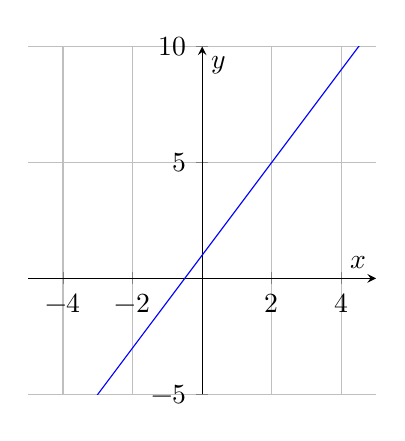
\begin{tikzpicture}
\begin{axis}[
    axis lines = middle,
    xlabel = $x$,
    ylabel = $y$,
    xmin=-5, xmax=5,
    ymin=-5, ymax=10,
    grid = major,
    width=6cm,
    height=6cm
]
\addplot[
    domain=-5:5,
    samples=100,
    color=blue
]
{2*x + 1};
\end{axis}
\end{tikzpicture}
\caption{Plot of the equation \( y = 2x + 1 \)}
\end{figure}
\end{frame}

\begin{frame}{Upward-sloping and downward-sloping lines}
\phantomsection\label{upward-sloping-and-downward-sloping-lines}
\begin{itemize}
\tightlist
\item
  If \(m > 0\), the line is ``upward-sloping'' or increasing.

  \begin{itemize}
  \tightlist
  \item
    As \(x\) increases, \(y\) also increases.
  \end{itemize}
\item
  If \(m < 0\), the line is ``downward-sloping'' or decreasing.

  \begin{itemize}
  \tightlist
  \item
    As \(x\) increases, \(y\) decreases.
  \end{itemize}
\end{itemize}

\begin{figure}
\centering
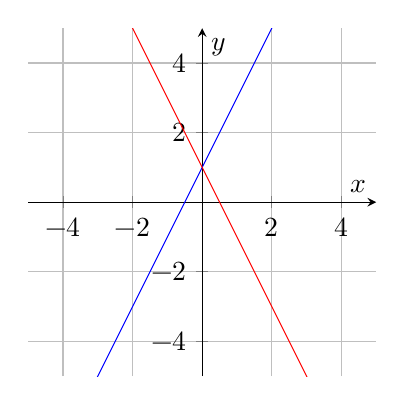
\begin{tikzpicture}
\begin{axis}[
    axis lines = middle,
    xlabel = $x$,
    ylabel = $y$,
    xmin=-5, xmax=5,
    ymin=-5, ymax=5,
    grid = major,
    width=6cm,
    height=6cm
]
\addplot[
    domain=-5:5,
    samples=100,
    color=blue
]
{2*x + 1};
\addplot[
    domain=-5:5,
    samples=100,
    color=red
]
{-2*x + 1};
\end{axis}
\end{tikzpicture}
\caption{Upward-sloping and downward-sloping lines}
\end{figure}
\end{frame}

\begin{frame}{Properties of slopes}
\phantomsection\label{properties-of-slopes}
\begin{itemize}
\item
  If \(m = 0\), the line is horizontal.

  \begin{itemize}
  \tightlist
  \item
    \(y\) does not change as \(x\) changes.
  \end{itemize}
\item
  If \(m = \infty\), the line is vertical.

  \begin{itemize}
  \tightlist
  \item
    \(x\) does not change as \(y\) changes.
  \end{itemize}
\item
  If \(m = 1\), the line has a 45-degree angle.
\item
  Lines with the same slope are parallel.
\item
  Lines with slopes that multiply to -1 are perpendicular.

  \begin{itemize}
  \tightlist
  \item
    This means that \(m_1 \cdot m_2 = -1\), or that
    \(m_1 = -\dfrac{1}{m_2}\) (the negative reciprocal).
  \end{itemize}
\end{itemize}
\end{frame}

\begin{frame}{How to find the equation of a line}
\phantomsection\label{how-to-find-the-equation-of-a-line}
\begin{enumerate}
\item
  If you know the slope \(m\) and a point \((x_1, y_1)\) on the line,
  you can use the point-slope form:

  \begin{itemize}
  \tightlist
  \item
    \(y - y_1 = m(x - x_1)\)
  \end{itemize}
\item
  If you know two points \((x_1, y_1)\) and \((x_2, y_2)\) on the line,
  you can use the slope formula to find \(m\) and then use
  \(y = mx + b\) to find \(b\).
\item
  If you know the slope \(m\) and the \(y\)-intercept \(b\), you can use
  \(y = mx + b\) directly (this is the slope-intercept form)
\end{enumerate}
\end{frame}

\begin{frame}{Graphing equation systems}
\phantomsection\label{graphing-equation-systems}
\begin{itemize}
\item
  To solve an equation system graphically, we graph both equations and
  find the point where they intersect.
\item
  The point of intersection is the solution to the system.
\item
  Example: graph the system
\end{itemize}

\begin{align*}
x + y &= 3 \\
2x - y &= 1
\end{align*}
\end{frame}

\begin{frame}{Graphing the system}
\phantomsection\label{graphing-the-system}
\begin{figure}
\centering
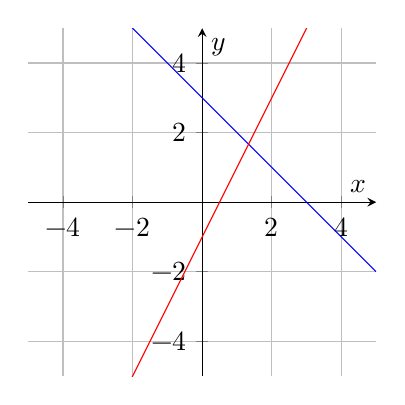
\begin{tikzpicture}
\begin{axis}[
    axis lines = middle,
    xlabel = $x$,
    ylabel = $y$,
    xmin=-5, xmax=5,
    ymin=-5, ymax=5,
    grid = major,
    width=6cm,
    height=6cm
]
\addplot[
    domain=-5:5,
    samples=100,
    color=blue
]
{3 - x};
\addplot[
    domain=-5:5,
    samples=100,
    color=red
]
{2*x - 1};
\end{axis}
\end{tikzpicture}
\caption{Graph of the system}
\end{figure}
\end{frame}

\begin{frame}{Systems with no solutions}
\phantomsection\label{systems-with-no-solutions}
\begin{itemize}
\tightlist
\item
  Sometimes, the lines are parallel and do not intersect.

  \begin{itemize}
  \tightlist
  \item
    This means that the system has no solution.
  \end{itemize}
\item
  How can we tell if two lines are parallel?

  \begin{itemize}
  \tightlist
  \item
    They have the same slope.
  \item
    The coefficients of \(x\) and \(y\) in the equations are
    proportional.
  \end{itemize}
\end{itemize}
\end{frame}

\begin{frame}{Systems with infinite solutions}
\phantomsection\label{systems-with-infinite-solutions}
\begin{itemize}
\tightlist
\item
  Sometimes, the lines coincide and intersect at every point.

  \begin{itemize}
  \tightlist
  \item
    This means that the system has infinite solutions.
  \end{itemize}
\item
  How can we tell if two lines coincide?

  \begin{itemize}
  \tightlist
  \item
    They have the same slope and the same \(y\)-intercept.
  \item
    The coefficients of \(x\) and \(y\) in the equations are
    proportional, and the constants are equal.
  \end{itemize}
\end{itemize}
\end{frame}

\begin{frame}{Graphic representations - systems with no solutions}
\phantomsection\label{graphic-representations---systems-with-no-solutions}
\begin{figure}
\centering
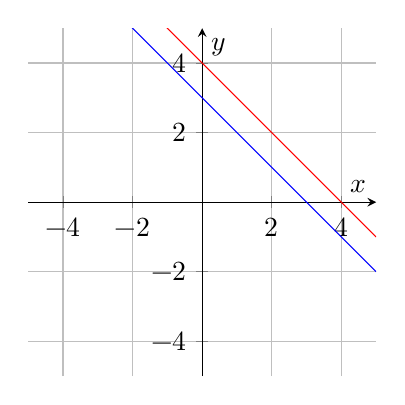
\begin{tikzpicture}
\begin{axis}[
    axis lines = middle,
    xlabel = $x$,
    ylabel = $y$,
    xmin=-5, xmax=5,
    ymin=-5, ymax=5,
    grid = major,
    width=6cm,
    height=6cm
]
\addplot[
    domain=-5:5,
    samples=100,
    color=blue
]
{3 - x};
\addplot[
    domain=-5:5,
    samples=100,
    color=red
]
{3 - x + 1};
\end{axis}
\end{tikzpicture}
\caption{Graph of a system with no solutions}
\end{figure}
\end{frame}

\begin{frame}{Graphic representations - systems with infinite solutions}
\phantomsection\label{graphic-representations---systems-with-infinite-solutions}
\begin{figure}
\centering
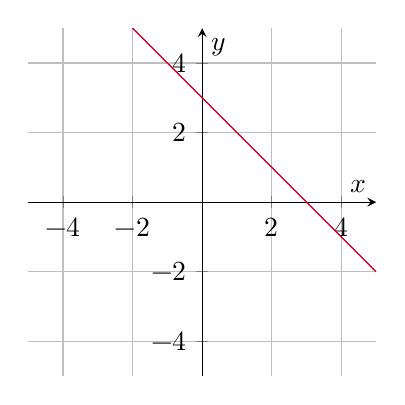
\begin{tikzpicture}
\begin{axis}[
    axis lines = middle,
    xlabel = $x$,
    ylabel = $y$,
    xmin=-5, xmax=5,
    ymin=-5, ymax=5,
    grid = major,
    width=6cm,
    height=6cm
]
\addplot[
    domain=-5:5,
    samples=100,
    color=blue
]
{3 - x};
\addplot[
    domain=-5:5,
    samples=100,
    color=red
]
{3 - x};
\end{axis}
\end{tikzpicture}
\end{figure}
\end{frame}

\begin{frame}{What happens when I try to solve a system that can't be
solved?}
\phantomsection\label{what-happens-when-i-try-to-solve-a-system-that-cant-be-solved}
\begin{itemize}
\tightlist
\item
  If you try to solve a system that has no solution, you will get a
  contradiction.

  \begin{itemize}
  \tightlist
  \item
    For example, you might find \(0 = 1\).
  \end{itemize}
\item
  If you try to solve a system that has infinite solutions, you will get
  an identity.

  \begin{itemize}
  \tightlist
  \item
    For example, you might find \(0 = 0\).
  \end{itemize}
\item
  In both cases, you cannot reach something like we're used to, like
  \(x = 3\) and \(y = 2\).
\end{itemize}
\end{frame}

\begin{frame}{More than two equations}
\phantomsection\label{more-than-two-equations}
\begin{itemize}
\tightlist
\item
  We can extend the concept of equation systems to more than two
  equations.

  \begin{itemize}
  \tightlist
  \item
    For example, a system of three equations in three variables.
  \end{itemize}
\item
  The same principles apply

  \begin{itemize}
  \tightlist
  \item
    Elimination
  \item
    Substitution
  \item
    Graphing
  \item
    Matrices (typically used for larger systems)
  \end{itemize}
\item
  For graphing, we need to consider more dimensions.

  \begin{itemize}
  \tightlist
  \item
    For a system of three equations in three variables, we need a
    three-dimensional space (3D), with \(x\), \(y\), and \(z\) axes.
  \end{itemize}
\end{itemize}
\end{frame}

\begin{frame}{Quadratic equations revisited}
\phantomsection\label{quadratic-equations-revisited}
\begin{itemize}
\tightlist
\item
  Quadratic equations are equations of the form \(y = ax^2 + bx + c\).

  \begin{itemize}
  \tightlist
  \item
    They represent parabolas in the Cartesian plane.
  \end{itemize}
\item
  The vertex of the parabola is given by \(x = -\dfrac{b}{2a}\).

  \begin{itemize}
  \tightlist
  \item
    This is where the parabola reaches its maximum or minimum.
  \item
    The vertex is the point where the parabola changes direction.
  \item
    It has coordinates \(\dfrac{-b}{2a}, f\left(\dfrac{-b}{2a}\right)\).
  \end{itemize}
\item
  The parabola opens upwards if \(a > 0\) and downwards if \(a < 0\).
\end{itemize}
\end{frame}

\begin{frame}{Graphing quadratic functions}
\phantomsection\label{graphing-quadratic-functions}
\begin{itemize}
\item
  To graph a quadratic function, the vertex is a good starting point.
\item
  If there are any roots or x-intercepts, they are also useful.

  \begin{itemize}
  \tightlist
  \item
    The roots are the points where the parabola crosses the x-axis.
  \item
    They are given by the solutions to the equation
    \(ax^2 + bx + c = 0\).
  \end{itemize}
\item
  Intercepts with the y-axis might be useful too.

  \begin{itemize}
  \tightlist
  \item
    The y-intercept is the point where the parabola crosses the y-axis.
  \item
    Solved by setting \(x = 0\) in the equation.
  \item
    They don't necessarily exist.
  \end{itemize}
\item
  Ultimately, might need to use a table of values to plot the parabola.
\end{itemize}
\end{frame}

\begin{frame}{Concave parabola}
\phantomsection\label{concave-parabola}
\begin{itemize}
\tightlist
\item
  A parabola that opens upwards is called \emph{concave}.

  \begin{itemize}
  \tightlist
  \item
    It has a minimum at the vertex.
  \end{itemize}
\end{itemize}

\begin{figure}
\centering
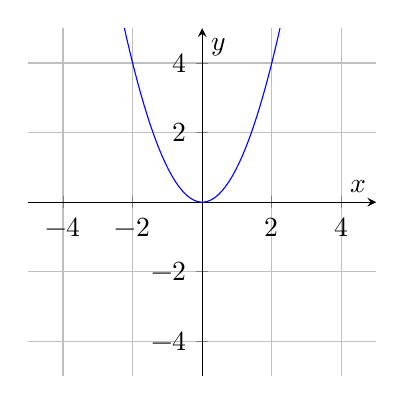
\begin{tikzpicture}
\begin{axis}[
    axis lines = middle,
    xlabel = $x$,
    ylabel = $y$,
    xmin=-5, xmax=5,
    ymin=-5, ymax=5,
    grid = major,
    width=6cm,
    height=6cm
]
\addplot[
    domain=-5:5,
    samples=100,
    color=blue
]
{x^2};
\end{axis}
\end{tikzpicture}
\caption{Concave parabola}

\end{figure}
\end{frame}

\begin{frame}{Convex parabola}
\phantomsection\label{convex-parabola}
\begin{itemize}
\tightlist
\item
  A parabola that opens downwards is called \emph{convex}.

  \begin{itemize}
  \tightlist
  \item
    It has a maximum at the vertex.
  \end{itemize}
\end{itemize}

\begin{figure}
\centering
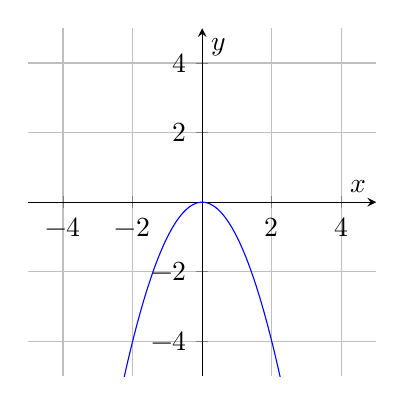
\begin{tikzpicture}
\begin{axis}[
    axis lines = middle,
    xlabel = $x$,
    ylabel = $y$,
    xmin=-5, xmax=5,
    ymin=-5, ymax=5,
    grid = major,
    width=6cm,
    height=6cm
]
\addplot[
    domain=-5:5,
    samples=100,
    color=blue
]
{-x^2};
\end{axis}
\end{tikzpicture}
\caption{Convex parabola}
\end{figure}
\end{frame}

\begin{frame}{Cubic equations/functions}
\phantomsection\label{cubic-equationsfunctions}
\begin{itemize}
\item
  Cubic equations are equations of the form
  \(y = ax^3 + bx^2 + cx + d\).

  \begin{itemize}
  \tightlist
  \item
    They represent cubic functions in the Cartesian plane.
  \end{itemize}
\item
  The graph of a cubic function is a curve that can have multiple
  inflection points.
\item
  The inflection points are points where the curve changes concavity.

  \begin{itemize}
  \tightlist
  \item
    Convex to concave or vice versa.
  \end{itemize}
\end{itemize}
\end{frame}

\begin{frame}{Graph of a cubic function}
\phantomsection\label{graph-of-a-cubic-function}
\begin{figure}
\centering
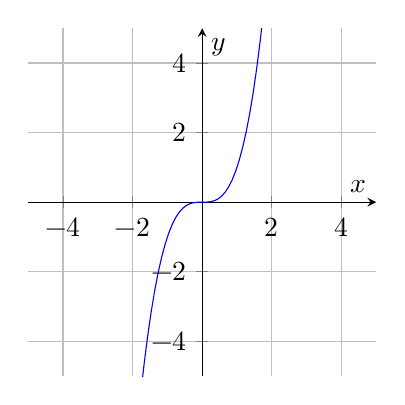
\begin{tikzpicture}
\begin{axis}[
    axis lines = middle,
    xlabel = $x$,
    ylabel = $y$,
    xmin=-5, xmax=5,
    ymin=-5, ymax=5,
    grid = major,
    width=6cm,
    height=6cm
]
\addplot[
    domain=-5:5,
    samples=100,
    color=blue
]
{x^3};
\end{axis}
\end{tikzpicture}
\caption{Graph of $x^3$}
\end{figure}
\end{frame}



\end{document}
